\documentclass{template/openetcs_article}
\usepackage {bsymb,b2latex}
\usepackage{lipsum,url,color}
\graphicspath{{./template/}{.}{./images/}}
\begin{document}
\frontmatter
\project{openETCS}

%Please do not change anything above this line
%============================
% The document metadata is defined below

%assign a report number here
\reportnum{OETCS}

%define your workpackage here
\wp{Work-Package 7: ``Toolchain''}


\newcommand{\true}{\ensuremath{true}}
\newcommand{\btext}[1]{{\it #1}}
\newcommand{\bvar}[1]{\btext{#1}}
\newcommand{\bevent}[1]{\btext{#1}}
\newcommand{\binv}[1]{\btext{#1}}
\newcommand{\bconst}[1]{\btext{#1}}
\newcommand{\bparam}[1]{\btext{#1}}
\newcommand{\bfunc}[1]{\btext{#1}}
\newcommand{\baxiom}[1]{\btext{#1}}
\newcommand{\btype}[1]{\btext{#1}}
\newcommand{\bguard}[1]{\btext{#1}}
\newcommand{\bmachine}[1]{\btext{#1}}
\newcommand{\bctx}[1]{\btext{#1}}

\author{Matthias Güdemann\\Systerel, France}

\affiliation{Systerel}

\title{Event-B Model of Subset 026, Section 3.13}

% define the coverart
\coverart[width=350pt]{chart}

\reporttype{Model Description}

%\begin{document}

\maketitle
\tableofcontents
\listoffiguresandtables
\newpage

This document describes a formal model of the requirements of section~3.13 of
the subset 026 of the ETCS specification 3.3.0~\cite{SRS-026-330}. This section
describes the speed and distance monitoring subsystem of ETCS.

The model is expressed in the formal language Event-B~\cite{abrial-eventB-Book}
and developed within the Rodin tool~\cite{rodin-handbook}. This formalism allows
an iterative modeling approach. In general, one starts with a very abstract
description of the basic functionality and step-wise adds additional details
until the desired level of accuracy of the model is reached. Rodin provides the
necessary proof support to ensure the correctness of the refined behavior.

In this document we present an Event-B model of the speed and distance
monitoring subsystem of ETCS. At first, we describe shortly the background of
Event-B, then the overall approach taken to model this section and finally
present the model in detail.

The section~3.13 of the SRS gives a very detailed description of the calculation
of many necessary values for speed and distance monitoring. As Event-B is a
system modeling approach, we give an abstract model of the system. The
calculations are abstracted as functions and the system ensures the correct
parameter flow to the functions. We illustrate the model decomposition
capabilities of Event-B and Rodin by decomposing the overall model into
different functional parts.


\begin{table}[ht]
  \centering
  \begin{tabular}[ht]{|l|l|}
    \hline
     &  \\
    \hline
  \end{tabular}
  \caption{Glossary}
  \label{tab:glossary}
\end{table}

\section{Short Introduction to Event-B}
\label{sec:short-intr-event}

The formal language Event-B is based on a set-theoretic approach. It is a
variant of the B language, with a focus on system level
modeling~\cite{abrial-eventB-Book}. An Event-B model is separated into a static
and a dynamic part.

The dynamic part of an Event-B model describes abstract state machines. The
state is represented by a set of state variables. A transition from one state to
another is represented by parametrized events which assign new values to the
state variables. Event-B allows unbounded state spaces. They are constrained by
invariants expressed in first order logic with equality which must be fulfilled
in any case. The initial state is created by a special initialization event.

The static part of an Event-B model is represented by contexts. These consist of
carrier sets, constants and axioms. The type system of a model is described by
means of carrier sets and constraints expressed by axioms.

Event-B is not only comprised of descriptions of abstract state machines and
contexts, but also includes a development approach. This approach consists of
iterative refinement of the machines until the desired level of detail is
reached. In the Rodin tool, proof obligations are automatically created which
ensure correct refinement.

Together with the machine invariants, the proof obligations for the refinement
are formally proven, creating proof trees. To accomplish this, there are
different options: many proof obligations can be discharged by automated provers
(e.g., AtelierB, NewPP, Rodin's SMT-plugin), but as the underlying logic is in
general undecidable, it is sometimes necessary to use the interactive proof
support of Rodin.

Any external actions, e.g., mode changes by the driver or train level changes
are modeled via parametrized events. Only events can modify the variables of a
machine. An Event-B model is on the system level, events are assumed to be
called from a software system into which the functional model is embedded. The
guards of the events assure that any event can only be called when appropriate.

\section{Modeling Strategy}
\label{sec:modeling-strategy}

The section~3.13 of the SRS describes the speed and distance monitoring together
with the necessary parameters and data. The model starts with an abstract
modeling of dataflow of the various intermediate calculated values. This model
is partitioned into functional parts, the model is decomposed using shared
variables and the respective sub-models are refined until the basic calculation
functions are reached.

\section{Model Overview}
\label{sec:model-overview}

The overview of the speed and distance monitoring is shown in
Fig.~\ref{fig:speed-distance-system} from the SRS.

\begin{figure}[ht]
  \centering
  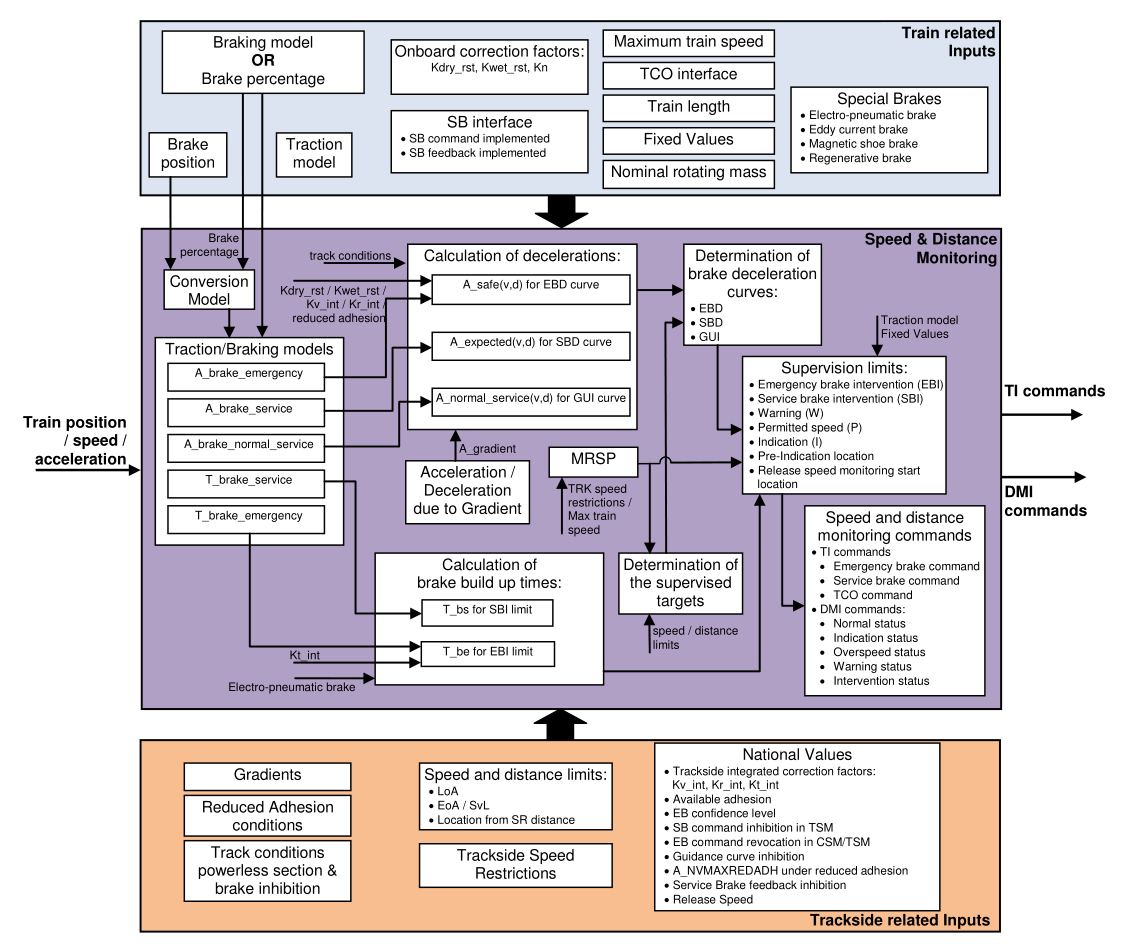
\includegraphics[width=.9\textwidth]{Overview_13_3}
  \caption{Speed and Distance Monitoring Overview~(\cite{SRS-026-330}~p.~85)}
  \label{fig:speed-distance-system}
\end{figure}

The on-board system comprises only the middle layer. The upper layer gives train
related inputs as parameters, the lower layer track related inputs. The system
itself takes the current position, speed and acceleration of the train and
computes commands for the train interface and for the driver machine
interface. For the train interface, this consists of the command for the service
and emergency brakes. For the driver machine interface this consists of the
status indication for the driver.

The Event-B modeling starts with machines describing the dataflow of all inputs,
outputs and intermediate values of the model. For example, the values that are
calculated for \bvar{T\_brake\_service} in \bmachine{Traction / Braking Models}
are written into a variable by an event that calculates then and these values
and are read as input by the event that calculates \bvar{T\_bs} for \bvar{SBI}
limit.

This approach is conducted for each intermediate value of the system until a
single machine is created with one variable for each intermediate value as well
as for each input and output. On this level of modeling, all events only define
the necessary input values and write a new value to their output variable. This
value is provided as event parameter on this abstraction level.

The next step is to decompose the single machine into different sub-machines, in
general one machine for each functional part of the model. This allows for model
structuring and complexity reduction for each machine. For this we use the Rodin
decomposition
plug-in~\footnote{\url{http://wiki.event-b.org/index.php/Decomposition_Plug-in_User_Guide}}
using the shared-variable decomposition
approach~\cite{silva2011decomposition}. This approach splits the set of events
of a machine into several disjoint sets and assigns one such set to each
sub-machine. It also allows to distribute the variables over several machines,
effectively implementing a shared variable distributed system.

The borders for the subsystem decomposition are shown in
Fig.~\ref{fig:system-decomposition}. The dashed lines show the separate
sub-machines. The dataflows that cross these lines are represented by the shared
variables of the decomposed model.

\begin{figure}[ht]
  \centering
  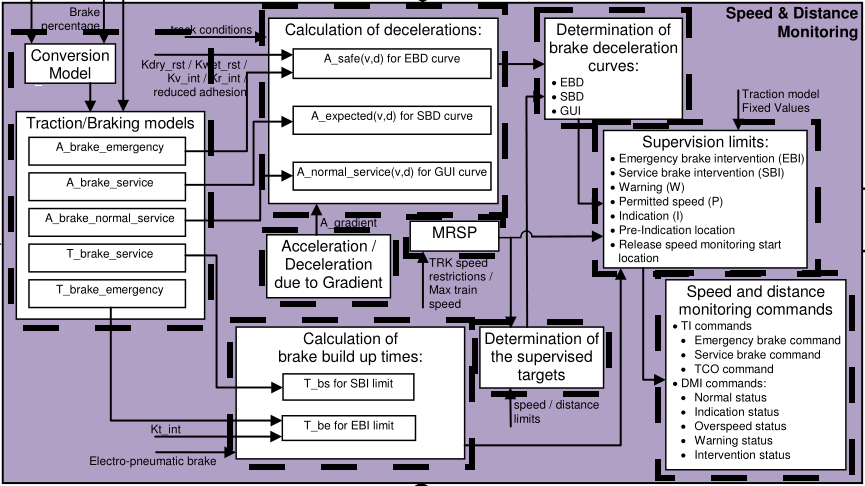
\includegraphics[width=.66\textwidth]{OverviewSelected}
  \caption{Decomposition of System}
  \label{fig:system-decomposition}
\end{figure}

Each of the sub-machines with its shared variables is then further refined until
the desired level of detail is reached. The overview of these refinements is
shown in Fig.~\ref{fig:machine-decompositon-overview}.

\begin{figure}[ht]
  \centering
  \vspace{5cm}
  \caption{Machine Decomposition Overview}
  \label{fig:machine-decompositon-overview}
\end{figure}

The context hierarchy also reflects this structuring. The contexts define the
data types for the intermediate values, as well as the functions that calculate
these values. These functions are generally not further refined in the Event-B
model, as this is not part of the system modeling.

\section{Model Benefits}
\label{sec:model-highlights}

The modeled section of the SRS provides many details for calculation of various
values. The main content from a system modeling point of view is the model. So
while in this case the same benefits from using Rodin as
for~\cite{Section-3-5-Rodin,Section-4-6-Rodin} are present, the main advantage
here is the model structuring facility.

\begin{itemize}
\item {\bf Model Decomposition} The shared variable model
  decomposition~\cite{silva2011decomposition} allows for decomposing an Event-B
  model and for separate refining of the machines of the resulting
  sub-models while retaining correctness of the refinement proofs.
\end{itemize}

\section{Detailed Model Description}
\label{sec:deta-model-descr}


\subsection{Context 0 - Train Inputs, TI and DMI command}
\label{sec:context-0-entities}

\begin{description}
\CONTEXT{c0\_train\_ti\_dmi\_commands}
\SETS
        \begin{description}
                \ItemY{ t\_locations }{all possible locations on track }
                \ItemY{ t\_speed }{train speed measurement }
                \ItemY{ t\_acceleration }{train acceleration }
                \ItemY{ t\_TI\_commands }{track interface commands }
                \ItemY{ t\_DMI\_commands }{driver machine interface commands }
                \ItemY{ t\_time }{ }
                \Item{ t\_train\_modes }
        \end{description}
\CONSTANTS
        \begin{description}
                \Item{ c\_emergency\_brake }
                \Item{ c\_service\_brake }
                \ItemY{ c\_TCO }{traction cut off}
                \ItemY{ c\_no\_command }{empty command}
                \Item{ c\_normal }
                \Item{ c\_indication }
                \ItemY{ c\_overspeed }{}
                \ItemY{ c\_warning }{}
                \ItemY{ c\_intervention }{}
                \Item{ c\_v0 }
                \Item{ c\_a0 }
                \ItemY{ c\_l0 }{}
                \Item{ c\_a\_brake0 }
                \ItemY{ c\_T\_brake0 }{}
        \end{description}
\AXIOMS
        \begin{description}
                \nItem{ axm1 }{ partition(t\_TI\_commands,\{ c\_no\_command\}
                  ,\{ c\_emergency\_brake\} ,\\ \hspace*{1.2cm} \{ c\_service\_brake\} ,\{ c\_TCO\} ) }\cmt{ }
                \nItem{ axm2 }{ partition(t\_DMI\_commands,\{ c\_normal\} ,\{
                  c\_indication\},\\ \hspace*{1.2cm}\{ c\_overspeed\} ,\{ c\_warning\} ,\{ c\_intervention\} ) }		\nItem{ axm3 }{ c\_v0 \in  t\_speed }		\nItem{ axm4 }{ c\_a0 \in  t\_acceleration }\cmt{ }
                \nItem{ axm5 }{ c\_l0 \in  t\_locations }		\nItem{ axm6 }{ c\_a\_brake0 \in  t\_speed \tfun  t\_acceleration }\cmt{		\\\hspace*{1,4 cm}  default brake profile }
                \nItem{ axm7 }{ c\_T\_brake0 \in  t\_time }\cmt{		\\\hspace*{1,4 cm}  default brake buildup time }
        \end{description}
\END
\end{description}


\subsection{Machine 0 - Basic Communication}
\label{sec:machine-0-basic}

\paragraph{Implemented Requirements}
\label{sec:impl-requ}

\begin{itemize}
\item each session allows for communication between two entities (cf.~§3.5.2.1)
\end{itemize}

%\begin{description}
\SEES{c0\_entities}
\VARIABLES
        \begin{description}
                \Item{ sessions }
        \end{description}
\INVARIANTS
        \begin{description}
                \nItem{ inv1 }{ sessions \subseteq  entities \setminus  \{ my\_entity\}  }
        \end{description}
\EVENTS
        \INITIALISATION\cmt{ }
                \begin{description}
                \BeginAct
                        \begin{description}
                        \nItem{ act1 }{ sessions :=  \emptyset  }
                        \end{description}
                \EndAct
                \end{description}
        \EVT {establish\_communication}
                \begin{description}
                \AnyPrm
                        \begin{description}
                        \ItemY{l\_partner }{ }
                        \end{description}
                \WhereGrd
                        \begin{description}
                        \nItemY{ grd1 }{ l\_partner \notin  sessions }{ }
                        \nItem{ grd2 }{ l\_partner \neq  my\_entity }
                        \end{description}
                \ThenAct
                        \begin{description}
                        \nItem{ act1 }{ sessions :=  sessions \bunion  \{ l\_partner\}  }
                        \end{description}
                \EndAct
                \end{description}
        \EVT {terminate\_communication}
                \begin{description}
                \AnyPrm
                        \begin{description}
                        \Item{l\_partner }
                        \end{description}
                \WhereGrd
                        \begin{description}
                        \nItem{ grd1 }{ l\_partner \in  sessions }
                        \end{description}
                \ThenAct
                        \begin{description}
                        \nItem{ act1 }{ sessions :=  sessions \setminus  \{ l\_partner\}  }
                        \end{description}
                \EndAct
                \end{description}
\END
\end{description}




\bibliographystyle{alpha}
\bibliography{openetcs}

\end{document}


%%% Local Variables:
%%% mode: latex
%%% TeX-master: t
%%% End:
